\documentclass[11pt,a4paper]{article}
\usepackage[top=3cm, bottom=2cm, left=2cm, right=2cm]{geometry}
\usepackage[utf8]{inputenc}
\usepackage{amsmath, amsfonts, amssymb}
\usepackage{siunitx}
\usepackage[brazil]{babel}
\usepackage{graphicx}
\usepackage[margin=10pt,font={small, it},labelfont=bf, textfont=it]{caption}
\usepackage[dvipsnames, svgnames]{xcolor}
\DeclareCaptionFont{MediumOrchid}{\color[svgnames]{MediumOrchid}}
\usepackage[pdftex]{hyperref}
\usepackage{natbib}
\bibliographystyle{plainnat}
\bibpunct{\textcolor{MediumOrchid}{\textbf{[}}}{\textcolor{MediumOrchid}{\textbf{]}}}{,}{s}{}{}
\usepackage{color}
\usepackage{footnote}
\usepackage{setspace}
\usepackage{booktabs}
\usepackage{multirow}
\usepackage{subfigure}
\usepackage{fancyhdr}
\usepackage{leading}
\usepackage{indentfirst}
\usepackage{wrapfig}
\usepackage{mdframed}
\usepackage{etoolbox}
\usepackage[version=4]{mhchem}
\usepackage{enumitem}
\usepackage{caption}
\usepackage{titlesec}
\usepackage{tcolorbox}
\usepackage{tikz}
\usepackage{LobsterTwo}
\usepackage[T1]{fontenc}
\usepackage{fontspec}
\usepackage{txfonts}
\usepackage[bottom]{footmisc}
\tcbuselibrary{skins,breakable}
\sisetup{output-decimal-marker={.}}

\makeatletter
\def\footnoterule{\kern-3pt\color{MediumOrchid}\hrule\@width0.6\textwidth height 0.8pt\kern2.6pt}
\makeatother

\renewcommand{\footnotelayout}{\itshape\color{MediumOrchid}}

\AtBeginEnvironment{equation}{\fontsize{13}{16}\selectfont}


\titleformat{\section}{\LobsterTwo\huge\color{CarnationPink}}{\thesection.}{1em}{}
\titleformat{\subsection}{\LobsterTwo\huge\color{CarnationPink}}{\thesubsection}{1em}{}
\titleformat{\subsubsection}{\bf\LobsterTwo\Large\color{MediumOrchid}}{\thesubsubsection}{1em}{}


\DeclareCaptionLabelFormat{figuras}{\textcolor{DarkTurquoise}{Figura \arabic{figure}}}
\captionsetup[figure]{labelformat=figuras}

\makeatletter
\renewcommand\tagform@[1]{\maketag@@@{\color{CarnationPink}(#1)}}
\makeatother

\renewcommand{\theequation}{Eq. \arabic{equation}}
\renewcommand{\thefigure}{Fig. \arabic{figure}}
\renewcommand{\thesection}{\textcolor{CarnationPink}{\arabic{section}}}

\setlist[itemize]{label=\textcolor{CarnationPink}{$\blacksquare$}}

\setlist[enumerate]{label=\textcolor{CarnationPink}{\arabic*.}, align=left, leftmargin=1.5cm}


\newcounter{exemplo}

\NewDocumentEnvironment{exemplo}{ O{} }{%
\allowbreak
\setlength{\parindent}{0pt}
  \begin{mdframed}[
  leftline=true,
  topline=false,
  rightline=false,
  bottomline=false,
  linewidth=2pt,
  linecolor=CarnationPink,
  frametitlerule=false,
  frametitlefont=\LobsterTwo\large\color{CarnationPink},
  frametitle={\color{CarnationPink}\LobsterTwo\large #1},
  ]
}{%
  \end{mdframed}
}

\setlength{\fboxsep}{5pt}
\setlength{\fboxrule}{1.5pt}
\usepackage{float}
\renewcommand{\thefootnote}{\alph{footnote}}
\usepackage{url}
\hypersetup{
	colorlinks=true,
	linkcolor=DarkTurquoise,
	filecolor=DarkTurquoise,      
	urlcolor=DarkTurquoise,
	citecolor=DarkTurquoise,
	pdftitle={Especialista em Física da Radioterapia}
}
\pagestyle{fancy}
\fancyhf{}
\renewcommand{\headrulewidth}{0pt}
\rfoot{\color{DarkTurquoise}\thepage \\ \LobsterTwo{\small\textcolor{CarnationPink}{@defDalila}}}

\title{\LobsterTwo\Huge{Radioterapia}}
\author{\LobsterTwo\Large{SRS e SBRT}\nocite{*}}
\date{\LobsterTwo\textit{Dalila Mendonça}}
\begin{document}
	\maketitle

\section{Introdução}

	A radiocirurgia estereotáxica (SRS) foi originalmente definida com o cumprimento de todas as seguintes condições:

	\begin{enumerate}[label=\textcolor{CarnationPink}{(\roman*)}]
		\item Tratamento com fração única;
		\item Alta dose por fração ($>$ 5Gy)
		\item Diâmetro do alvo $<$ 3.5 cm no cérebro;
		\item Precisão na entrega da dose $<$ 1 mm como definido pelo teste de Winston-Lutz\cite{lutz1988system};
		\item Nenhuma margem para PTV ou ITV é usada; podendo ser utilizada as margens para o CTV, mas no geral trata apenas o GTV; 
	\end{enumerate}

	A SRS foi posteriormente expandida para incluir também tratamentos de lesões na coluna vertebral com fração única e também para incluir tratamentos fracionados. A definição atual inclui:

	\begin{enumerate}[label=\textcolor{CarnationPink}{(\roman*)}]
		\item Tratamentos de 1 até 5 frações;
		\item Alta dose por fração (acima de 5 Gy);
		\item Diâmetro do alvo menor que 3.5 cm no sistema nervoso central (SNC  - crânio ou medula);
		\item Precisão na entrega da dose $<$ 1 mm como definido pelo resultado do teste end-to-end;
	\end{enumerate}

	A SBRT (Stereotactic Body Radiation Therapy), as vezes também chamada de SABRT (Stereotactic Ablative Radiation Therapy) é definida pelas seguintes condições:

	\begin{enumerate}[label=\textcolor{CarnationPink}{(\roman*)}]
		\item Tratamentos de 1 a 5 frações (Até 8 frações no Canadá);
		\item Altas doses por fração (acima de 5 Gy);
		\item Tamanho do alvo de até 4 cm de diâmetro para lesões no pulmão ou de 5 cm até 7 cm de diâmetro para alvos localizados nas cavidades torácicas e abdominais.
		\item Precisão na entrega do tratamento $<$ 1.5 mm até 2 mm definidas pelos resultados dos testes end-to-end;
		\item As margens para o ITV e para o PTV são utilizadas para compensar a movimentação intra-fração e inter-fração e deformações. A maioria dos alvos, exceto a próstata, necessitam de um gerenciamento do movimento respiratório.
	\end{enumerate}

\section{Requerimentos Técnicos}

	As altas doses e os acentuados gradientes de dose entregues em poucas frações nos tratamentos de SRS e SBRT resultam eum uma margem de erro muito menor que o os fracionamentos de radioterapia convencionais. Uma máquina utilizada para a tratamentos de SRS/SBRT deve, portanto, atender no mínimo aos seguintes requisitos técnicos mais rigorosos:

	\begin{enumerate}[label=\textcolor{CarnationPink}{(\roman*)}]
		\item A máquina deve atender às tolerâncias mecânicas descritas no TG-142;
		\item Os campos pequenos devem estar comissionados;
		\item Recursos de orientação pro imagem ( ou frame);
		\item Resultados do teste end-to-end (E2E) $<$ 1 mm e resultados do QA entrega (DQA) $<$3\%/2 mm.
		\item Técnicas de gerenciamento do movimento respiratório;
	\end{enumerate}

	O teste E2E é uma adaptação do teste Winston-Lutz para a era do SRS/SBRT frameless guiada por imagem. Idealmente, no teste E2E, cada uma das etapas deve ser realizada pelo(s) membro(s) da equipe envolvidos no tratamento que desempenharão esta mesma etapa no tratamento de um paciente. A realização de um teste E2E da maneira apresentada a seguir como parte do processo de comissionamento, pode ajudar a esclarecer o fluxo de tratamento e o fluxo de informações e também pode servir como uma ferramenta para desenvolver o conjunto inicial de políticas e procedimentos (POP):

	\begin{enumerate}[label=\LobsterTwo\textbf{\textcolor{CarnationPink}{\arabic*${}^\circ$}}]
		\item \LobsterTwo\textbf{\textcolor{CarnationPink}{$\star$ Físico Médico $\star$}} Um phantom  antropomórfico apropriado para o local de tratamento, equipado com fiduciais para localização semelhante ao que será usado em um paciente, é carregado com ferramentas de dosimetria in vivo, como dosímetro termoluminescente (TLD), detector luminescente opticamente estimulado (OSLD), metal- transistores de efeito de campo semicondutores de óxido (MOSFETs), gel ou filme (físico médico).
		
		\item \LobsterTwo\textbf{\textcolor{DarkTurquoise}{$\star$ Técnico $\star$}} O phantom é imobilizado e adquirida sua imagem, usando os mesmos dispositivos de imobilização e protocolos de aquisição que seriam usados para o paciente.
		
		\item \LobsterTwo\textbf{\textcolor{MediumOrchid}{$\star$ Médico $\star$}} As imagens são importadas para o sistema de planejamento de tratamento e o alvo oculto é contornado.
		
		\item \LobsterTwo\textbf{\textcolor{DarkTurquoise}{$\star$ Dosimetrista $\star$}}Um plano de tratamento é desenvolvido cumprindo as restrições de dose prescritas .
		
		\item \LobsterTwo\textbf{\textcolor{MediumOrchid}{$\star$ Médico $\star$}}O plano é assinado e revisado.
		
		\item \LobsterTwo\textbf{\textcolor{DarkTurquoise}{$\star$ Dosimetrista $\star$}} A documentação do plano é gerada e o plano é exportado para a unidade de tratamento.
		
		\item \LobsterTwo\textbf{\textcolor{CarnationPink}{$\star$ Físico Médico $\star$}} Uma segunda verificação, cálculo da unidade de monitor secundário (MU) e medições de controle de qualidade específicas do paciente, se aplicável, são realizadas.
		
		\item \LobsterTwo\textbf{\textcolor{DarkTurquoise}{$\star$ Técnico $\star$}}O tratamento é entregue .
		\item \LobsterTwo\textbf{\textcolor{CarnationPink}{$\star$ Físico Médico $\star$}} O resultado da medição da dose é analisado.
	\end{enumerate}


\section{Políticas e Procedimentos}

	Antes de iniciar um programa de SRS/SBRT, uma série de políticas e procedimentos P\&Ps devem ser desenvolvidas uma configuração multidisciplinar de todos os prestadores de cuidados envolvidos. Para determinar quais P\&Ps são necessários, um fluxograma do paciente pode ser uma ferramenta útil. Este fluxograma também servirá como uma ferramenta de controle de qualidade para garantir que todos os membros da equipe de tratamento do paciente entendam seu papel no processo de atendimento, a ordem das etapas do atendimento e o fluxo de informações.

	A \ref{fig:srsPop} descreve um exemplo de um conjunto de P\&Ps para atender às diretrizes de credenciamento da prática no American College of Radiology (ACR) e ao escopo das diretrizes da prática da Canadian Association of Radiation Oncologists (CARO) para recomendações SBRT de pulmão, fígado e coluna. O white paper da ASTRO a respeito das considerações de qualidade e segurança na SBRT enfatiza que a SRS/SBRT não são uma única técnica/modalidade e que o conhecimento em uma área-alvo anatômica não constitui um conhecimento em outros locais. Portanto, é necessário desenvolver procedimentos específicos para a tecnologia em uso na instituição, bem como procedimentos específicos para os locais da doença.

	\begin{figure}[h]
		\centering
		\fcolorbox{DarkTurquoise}{white}{%
			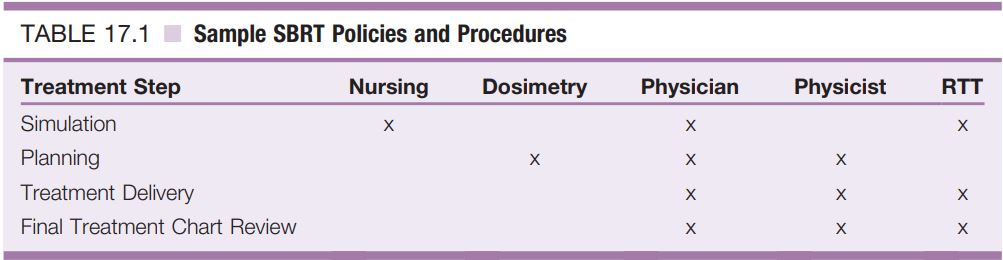
\includegraphics[width=0.9\textwidth]{Imagens/srsPop.JPG}
		}%
		\caption{Exemplo de Políticas e Procedimentos para SBRT.}
		\label{fig:srsPop}
	\end{figure}

	Os P\&Ps devem ser testados usando um cenário simulado do tratamento do paciente, preferencialmente incluindo a aquisição de imagens e o planejamento e entrega de um plano de tratamento em um phantom. Após o tratamento dos primeiros pacientes, as P\&Ps devem ser revisadas. Após a revisão inicial, os P\&Ps devem ser revisados e, se aplicável, atualizados anualmente.

	Em vez de fichários em vários locais, que são difíceis de manter atualizados, um sistema eletrônico deve ser usado para armazenar centralmente os manuais de P\&P. O P\&P deve ser acessível a todos os membros do departamento de Radioterapia, deve ser acessível a partir da maioria das estações de trabalho clínicas e oferecer rastreamento de versão e recursos de aprovação para identificar facilmente a iteração mais atualizada do P\&P. 


\section{Staffs}

	A implementação e manutenção de um programa SRS/SBRT requer pessoal adequado para alcançar tratamentos seguros e de alta qualidade. O estudo Abt de 2008 fornece estimativas medianas de trabalho para procedimentos SRS/SBRT, uma vez que eles são estabelecidos na rotina clínica. O white paper da American Society for Radiation Oncology (ASTRO) a respeito das considerações de qualidade e segurança para a técnica de SBRT afirma que “níveis adequados de especialização da equipe estão intimamente relacionados a uma redução de erros médicos”. Além disso, recomenda fornecer pessoal adequadamente treinado, oportunidades de educação continuada e “tempo suficiente para que a equipe desempenhe suas tarefas necessárias, sem estresse ou fadiga indevidos\dots”.

	As diretrizes práticas do ACR sobre SBRT e SRS, bem como o white paper da ASTRO sobre considerações de qualidade e segurança em SBRT, recomendam que um físico médico qualificado (QMP) com treinamento específico em SBRT seja responsável pelos aspectos técnicos de SRS/SBRT. Um QMP com a finalidade de supervisionar o SRS/SBRT é definido como um indivíduo que recebeu certificação do conselho em física médica terapêutica ou subespecialidade equivalente pelo American Board of Radiology (ABR), Canadian College of Medical Physics (CCMP) ou American Board de Física Médica (ABMP). Essa recomendação foi reforçada em comparação com as diretrizes de prática agora aposentadas, nas quais todas as subespecialidades da física médica foram listadas como apropriadas para realizar SRS/SBRT. As responsabilidades do QMP incluem todos os aspectos técnicos do SRS/SBRT, estabelecendo uma lista de verificação de controle de qualidade (QC) para todo o processo de tratamento, supervisionando o planejamento do tratamento, segunda verificação de MU e QA de entrega específica do paciente e comunicação com o oncologista de radiação.

	O escopo da diretriz prática CARO para SBRT de pulmão, fígado e coluna espera que o QMP comunique ao oncologista de radiação quando as limitações e suposições feitas em cada etapa do processo de tratamento forem alcançadas. Isso requer uma compreensão profunda por parte do QMP das limitações e suposições usadas no processo. Além disso, espera-se que o QMP revise todos os planos de tratamento SBRT antes da entrega. Espera-se que o QMP tenha treinamento específico em SBRT por meio de um curso educacional ou mentoria. O QMP também deve ser versado em diretrizes publicadas (por exemplo, AAPM TGs aplicáveis) que orientam a implementação de QA rigoroso para SRS/SBRT.

\section{Seleção do Paciente e Desenvolvimento de Protocolos de Tratamento}

	O AAPM TG-101, \textit{\textbf{``Stereotactic Body Radiation Therapy''}} recomenda inscrever os pacientes SRS/SBRT em um estudo clínico. Se isso não for viável, recomenda-se tratar os pacientes por estudo ou diretrizes publicadas revisadas por pares. Qualquer desvio significativo dos protocolos de ensaios clínicos ou de guidelines publicados deve ser estruturado como um estudo prospectivo sob revisão do IRB. Essas recomendações são confirmadas pelo escopo das diretrizes práticas do CARO para SBRT de pulmão, fígado e coluna. O white paper da ASTRO sobre considerações de qualidade e segurança no SBRT recomenda a coleta de uma biblioteca de estudos publicados revisados por pares relevantes para os locais específicos da SBRT e que a instituição documente claramente os planos para seleção de pacientes, planejamento de tratamento e administração de tratamento antes de iniciar um programa de SRS/SBRT.

\section{Imagem de Simulação}

	Em procedimentos de SRS utilizando frame ou SBRT de coluna, assume-se que a estrutura-alvo não se move em relação ao sistema de coordenadas estereotáxicas. Se houver suspeita de possíveis alterações na localização do tumor ou alterações na posição do quadro (por exemplo, deslocamento), os métodos utilizando frame podem e devem ser complementados com imagens pré-tratamento. Em SRS/SBRT frameless, se forem usados marcadores fiduciais para localizar o tumor, os marcadores fiduciais devem ser colocados adequadamente dentro ou ao redor do tumor para obter a precisão necessária. Pontos de referência anatômicos, como estruturas ósseas ou, no caso de tumores pulmonares, o próprio tumor também podem ser usados diretamente como fiduciais.

	Para SRS de coluna, os guidelines da CARO para SBRT de pulmão, fígado e coluna recomenda o uso de um sistema de imobilização de corpo quase rígido (\textit{``near-rigid body immobilization system''}) para minimizar o movimento intrafração. Para sistemas de entrega capazes de gerar imagens e corrigir o movimento do paciente intrafração, os requisitos para o sistema de imobilização podem ser menos rigorosos. Para todos os procedimentos SRS/SBRT frameless, o guideline do ACR sobre SBRT recomenda que a posição do paciente seja confortável o suficiente para que ele fique imóvel durante todo o procedimento.

	A imagem de simulação com alta resolução é a base para a identificação do GTV e, portanto, para a precisão do contorno. Para entrega SRS/SBRT guiada por imagem, a resolução da aquisição de simulação influenciará a precisão da orientação por imagem durante o tratamento.

	\begin{itemize}
		\item Para SRS, é necessária uma espessura de corte axial $<$1.25 mm.
		\item Em SBRT, onde tumores e OARs são geralmente maiores, uma espessura de corte <3 mm é recomendada pelo AAPM TG-101.
		\item os guidelines da CARO para SBRT de pulmão, fígado e coluna recomenda uma espessura de corte da TC $<$2.5 mm para coluna e $<$3 mm para fígado. 
	\end{itemize}

	Geralmente, uma tomografia computadorizada é utilizada como a modalidade de imagem baseline para o planejamento do tratamento SRS/SBRT. A TC fornece informações precisas sobre a densidade eletrônica, embora a influência do uso de contraste durante a simulação na precisão do cálculo da dose deva ser investigada. As imagens de TC geralmente têm uma distorção espacial muito baixa. Além disso, a imagem de TC 4D é uma possibilidade para corresponder ao gerenciamento planejado do movimento respiratório durante o tratamento.

	O AAPM TG-101 recomenda um tamanho longitudinal para aquisição da imagem de 5 a 10 cm superior e inferior além das bordas do tratamento ou de 15 cm se feixes não coplanares forem usados. Todos os OARs devem ser incluídos e avaliados usando histogramas de dose-volume (DVH). 

	Se o alvo ou OAR não puder ser identificado com precisão devido a artefatos na imagem, a SRS/SBRT não deve ser considerada uma opção de tratamento segura. Os guidelines da CARO para SBRT de pulmão, fígado e coluna sugere uma imagem de ressonância magnética (MRI) (axial volumétrica ponderada em T1 e T2) estendendo-se além de um corpo vertebral acima e abaixo da região alvo em tratamentos de SRS de coluna. Os guidelines da ACR para SBRT recomendam a investigação de todas as imagens digitais em busca de distorções espaciais que possam surgir nas cadeias de imagem.

	Considerações adicionais para simulação e geração de imagens são:

	\begin{itemize}[label=\textcolor{CarnationPink}{$\blacktriangleright$}]
		\item \textcolor{DarkTurquoise}{\textbf{Contraste:}} Os guidelines da CARO para SBRT de pulmão, fígado e coluna recomendam o uso de ressonância magnética multifásica com contraste de gadolínio intravenoso para câncer de fígado. Para o câncer hepático primário, recomenda-se a imagem da fase arterial tardia, enquanto as metástases hepáticas são melhor visualizadas na fase venosa. Para o pulmão, a recomendação é usar contraste para lesões mediais ou próximas a atelectasias\footnote{A atelectasia é uma condição médica em que uma parte ou a totalidade de um pulmão colapsa ou se torna parcialmente colapsado. Isso ocorre quando os alvéolos pulmonares, que são pequenos sacos de ar onde ocorre a troca de oxigênio e dióxido de carbono durante a respiração, se esvaziam ou restringem devido a diferentes razões: quando há um bloqueio nas vias aéreas que impede o ar de chegar aos alvéolos (atelectasia de reabsorção), quando uma estrutura fora do pulmão exerce pressão sobre ele (atelectasia compressiva), quando o tecido pulmonar se retrai devido a cicatrizes ou doenças pulmonares crônicas (atelectasia por contração) ou quando há um bloqueio mecânico das vias aéreas dentro do pulmão (atelectasia por obstrução). }, mas o contraste pode ser evitado principalmente para lesões mais periféricas.
		
		\item \textcolor{DarkTurquoise}{\textbf{Fusão de Imagem:}} Para muitos alvos SBRT, a imagem de TC não é a ferramenta diagnóstica ideal para definir uma lesão. Para lesões cerebrais, a ressonância magnética é a modalidade de imagem de escolha. No pulmão e no abdome, a tomografia por emissão de pósitrons (PET) é usada, geralmente como PET/CT. Se conjuntos de imagens secundárias para a simulação CT forem usados para definição de alvo, a transferência correta desses conjuntos de imagens para o sistema de planejamento de tratamento deve ser verificada. Além disso, os algoritmos de fusão -- incluindo seus pontos fortes e fracos -- devem ser bem compreendidos e testados. Especialmente ao usar o registro de imagens deformáveis, é necessário que o físico e o médico tenham uma compreensão clara das incertezas potencialmente grandes envolvidas no processo de fusão. O AAPM TG-132, \textit{\textbf{``Use of Image Registration and Data Fusion Algorithms and Techniques in Radiotherapy Treatment Planning''}} fornecem orientações mais detalhadas sobre a fusão de imagens.
		
		\item \textcolor{DarkTurquoise}{\textbf{Gerenciamento do Movimento Respiratório:}} Deve ser considerada para lesões no pulmão e na cavidade abdominal.
		
	\end{itemize}
	
\section{Margens}

	Tradicionalmente, não são usadas margens explícitas do CTV na SRS, com exceção do tratamento de cavidades de ressecção no cérebro, onde algumas instituições adicionam uma margem para o CTV de 2 mm. Para o tratamento de SRS de metástases da coluna vertebral, o International Spine Radiosurgery Consortium publicou diretrizes detalhadas de contorno para cenários comuns em radiocirurgia da coluna. 

	A fórmula de margem de van Herk é frequentemente usada para determinar as margens de PTV em regimes de fracionamento de tratamento tradicionais. No entanto, baseia-se na suposição de um número suficientemente alto de frações para que uma estatística de Poisson para erros aleatórioa seja válida e também pressupõe o uso de radioterapia conformacional 3D. Houve esforços para adaptar a fórmula de van Herk para SRS/SBRT e estudos baseados em Monte Carlo\cite{herschtal2012calculating} foram publicados com respeito ao tamanho da margem especificamente para SRS/SBRT. Como a SRS/SBRT frameless ainda é uma modalidade ``relativamente'' nova, recomenda-se usar margens com base nas recomendações de grupos de ensaios clínicos ou, se não estiverem disponíveis, consultar estudos clínicos prospectivos publicados usando processos e equipamentos semelhantes (\ref{fig:srsMargens}).

	\begin{figure}[h]
		\centering
		\fcolorbox{DarkTurquoise}{white}{%
			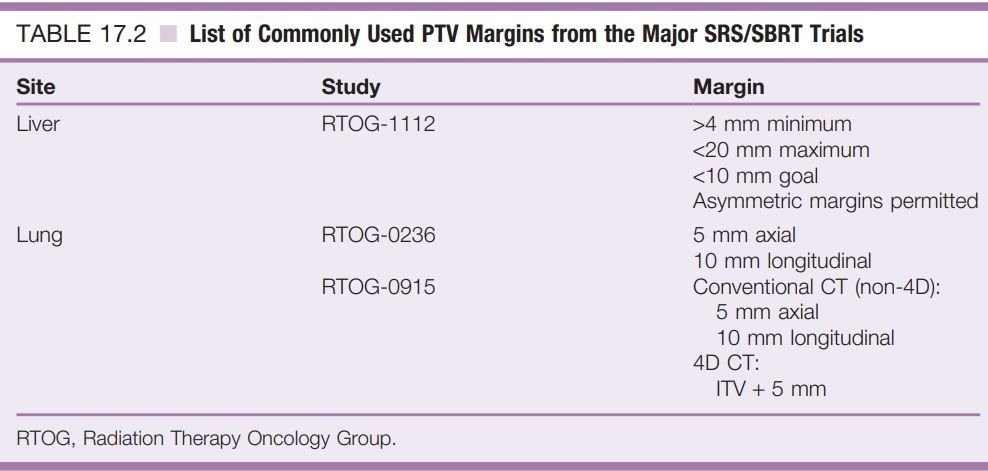
\includegraphics[width=0.9\textwidth]{Imagens/srsMargens.JPG}
		}%
		\caption{Lista de margens para o PTV comumente usadas nos principais ensaios de SRS/SBRT.}
		\label{fig:srsMargens}
	\end{figure}

	No pulmão, a CARO recomenda o uso de uma imagem de projeção da intensidade máxima (MIP) para o delineamento do ITV, mas não para o cálculo da dose. Alguns grupos, no entanto, observaram que as imagens MIP não fornecem qualidade de imagem adequada na presença de movimento respiratório e, portanto, utilizam aquisições 4D-CT para delinear o GTV.


\section{Constraints de Dose e Planejamento do Tratamento}

	O white paper da ASTRO sobre considerações de qualidade e segurança em SBRT recomenda que o sistema de planejamento seja capaz de suportar multimodalidade e dados de imagens multidimensionais de TC, RM e PET (\ref{fig:srsDoses} e \ref{fig:srsConstraints}). 

	\begin{figure}[!hbt]
		\centering
		\fcolorbox{DarkTurquoise}{white}{%
			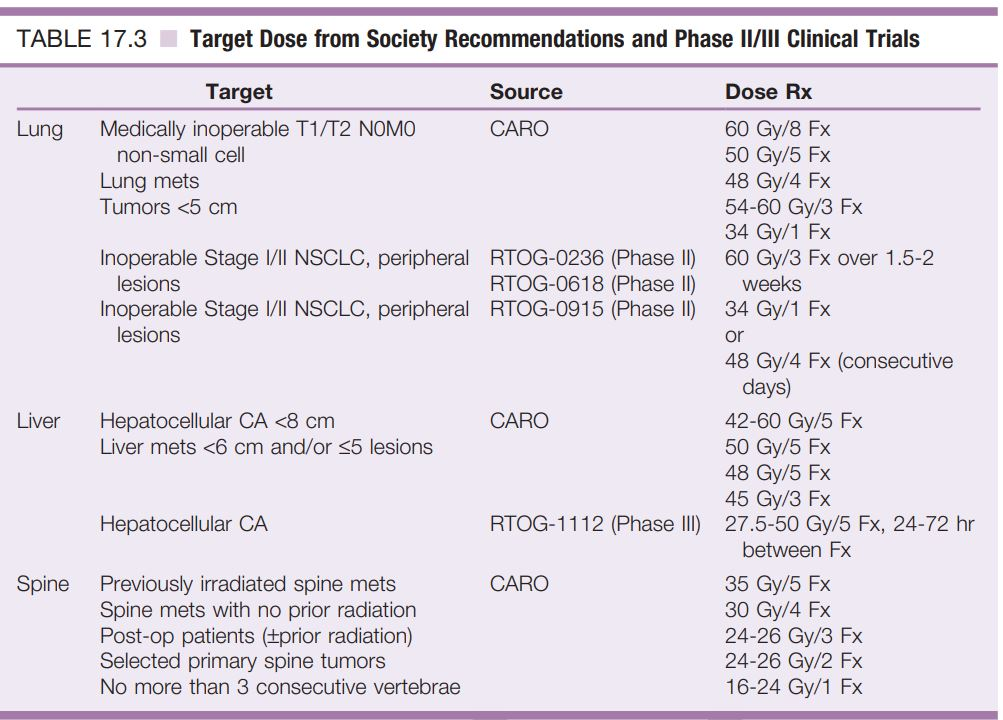
\includegraphics[width=0.8\textwidth]{Imagens/srsDoses.JPG}
		}%
		\caption{Dose Alvo das Recomendações da ASTRO e Ensaios Clínicos de Fase II/III.}
		\label{fig:srsDoses}
	\end{figure}

	\begin{figure}[!hbt]
		\centering
		\subfigure{
			\fcolorbox{DarkTurquoise}{white}{%
				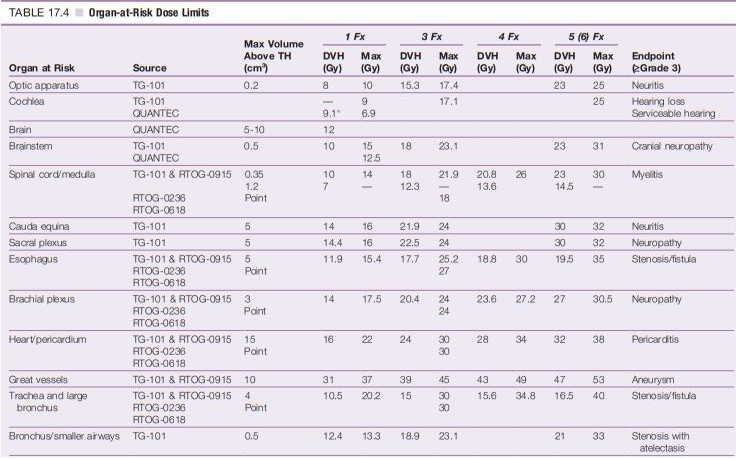
\includegraphics[width=0.67\textwidth]{Imagens/srsConstraints1.JPG}
			}} \\
		\subfigure{
			\fcolorbox{DarkTurquoise}{white}{%
				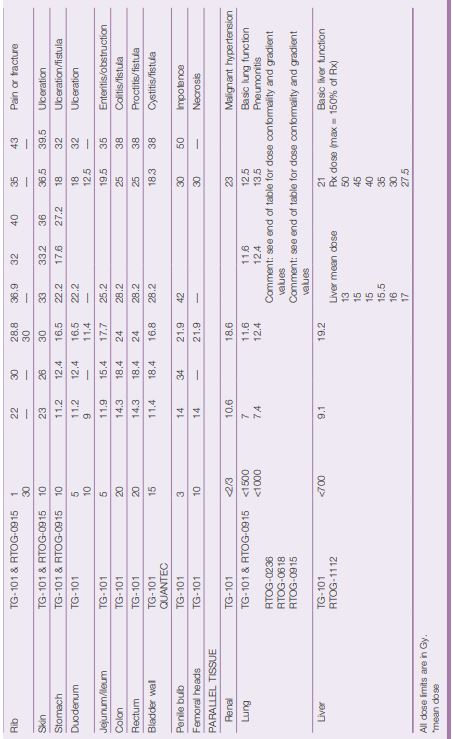
\includegraphics[width=0.67\textwidth]{Imagens/srsConstraints2.JPG}
			}} \\ %
			\subfigure{
			\fcolorbox{DarkTurquoise}{white}{%
				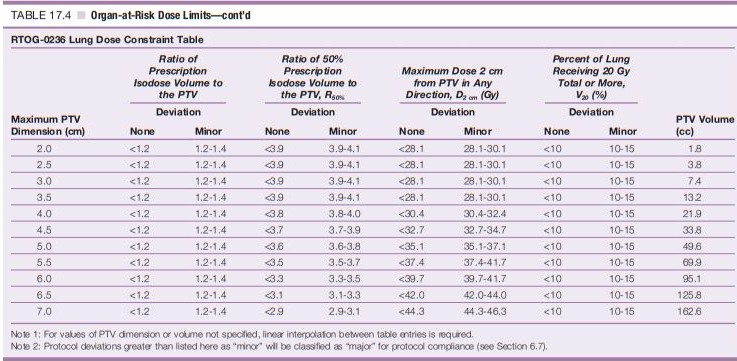
\includegraphics[width=0.67\textwidth]{Imagens/srsConstraints3.JPG}
			}} \\ %
		\caption{Constraints para os OARs}
		\label{fig:srsConstraints}
	\end{figure}


\subsection*{RTOG e Outros Protocolos}

	O RTOG apresentou um constraint de compactação de $PTV + 2 \text{ cm}$ para limitar o volume de dose intermediária dos OARs. Indiretamente, o uso de um constraint de compactação força o uso de feixes múltiplos, diminuindo o risco de toxicidade cutânea causada por pontos quentes na entrada do feixe distantes do alvo. Pontos quentes dentro do alvo não são apenas aceitáveis, mas frequentemente desejáveis; por exemplo, alguns protocolos de tratamento de SBRT pulmonar especificam um ponto quente de 25\% a 30\% dentro do GTV. O gradiente de dose fora do alvo deve ser acentuado (por exemplo, de 1 Gy/mm na coluna SRS até 16 Gy/mm para SRS de neuralgia dos trigêmeos). Para calcular com precisão a dose considerando os gradientes de dose acentuados, a grade de cálculo de dose do sistema de planejamento de tratamento deve ser definida para a resolução mais alta que mantenha o tempo de cálculo clinicamente razoável. Neste momento, é $\leq$ 2 mm para a maioria dos sistemas de planejamento de tratamento e 2\% para a maioria dos sistemas de planejamento de tratamento baseados em MC.

	A subdosagem do PTV pode ser necessária para proteger os órgãos críticos adjacentes ao alvo. Um exemplo típico seria na SRS de coluna, onde o limite de dose para a medula combinado com o gradiente de dose atualmente alcançável para feixes de fótons quase sempre exigirá que uma pequena área posterior do corpo vertebral seja subdosada.

	Os tumores pulmonares, mas também os tumores da cabeça e pescoço e do cérebro, localizam-se perto de grandes heterogeneidades teciduais. A capacidade do sistema de planejamento de tratamento de calcular com precisão a dose e os gradientes de dose para um pequeno campo de tratamento deve ser avaliada e documentada. O AAPM TG-65, \textit{\textbf{``Tissue Inhomogeneity Corrections for Megavoltage Photon Beams''}}\cite{papanikolaou2004tissue}, fornece recomendações específicas sobre o uso de cálculos de heterogeneidade. O white paper da ASTRO recomenda que o sistema de planejamento de tratamento corrija a falta de homogeneidade do tecido com precisão suficiente, embora não estabeleça um limite específico além de excluir a maioria dos algoritmos pencil beam para essa finalidade. O white paper também recomenda o controle de qualidade da correção da heterogeneidade durante o processo de comissionamento usando um phantom apropriado.

	Várias opções de planejamento de tratamento estão disponíveis, dependendo do uso de colimação (cones ou MLC), bem como do sistema de entrega. A \ref{fig:srsTecnicas} lista as configurações de feixe de tratamento usadas no planejamento de SBRT.

	\begin{figure}[h]
		\centering
		\fcolorbox{DarkTurquoise}{white}{%
			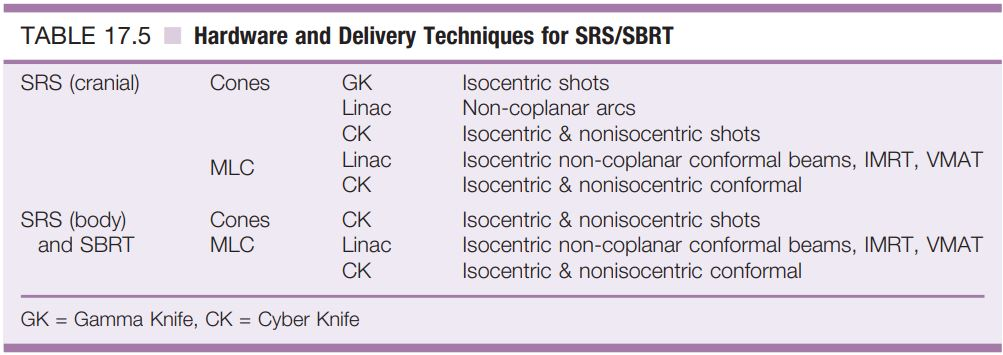
\includegraphics[width=0.8\textwidth]{Imagens/srsTecnicas.JPG}
		}%
		\caption{Hardware e Técnicas de Entrega para SRS/SBRT.}
		\label{fig:srsTecnicas}
	\end{figure}

	Ao usar feixes não coplanares, é recomendável realizar uma simulação de entrega do tratamento para identificar possíveis riscos de colisão. Os guidelines da CARO recomenda o uso de índices de conformidade, pois eles são úteis ao avaliar a qualidade geral do plano. Os guidelines da ACR sobre SBRT recomenda ter um processo documentado para comissionar um sistema de planejamento de tratamento para uso clínico para SRS/SBRT e monitoramento contínuo do desempenho do sistema de planejamento de tratamento.

\section{Entrega do Tratamento}

	Para tratamentos SRS/SBRT framelessa, sistemas de orientação por imagem precisos devem ser usados para o setup do paciente e gerenciamento de movimento intrafração. As opções de orientação por imagem incluem registro 2D-3D usando raios X ortogonais, registro de imagem kV-MV e tomografia computadorizada de feixe cônico (CBCT) kV ou MV. Mais recentemente, tecnologias não ionizantes usando luz visível (VisionRT), rastreamento eletromagnético (Calypso) ou ultrassom (Clarity) tornaram-se disponíveis para uso clínico. O AAPM TG-101 recomenda definir níveis de ação para desvios de translação e rotações acima dos quais a o posicionamento do paciente deve ser corrigido. 

	O guideline da ACR sobre SBRT e SRS recomenda testar o sistema de orientação por imagem e o sistema de administração do tratamento de maneira integrada para verificar se eles funcionam juntos com precisão durante o processo de entrega do tratamento. Os sistemas devem demonstrar a capacidade de localizar e posicionar um alvo oculto e subsequentemente irradiar o alvo com uma precisão especificada. Este tipo de teste é parte integrante de um teste E2E. Além disso, o AAPM TG-142 recomenda a verificação diária da concordância entre o sistema de imagem e o sistema de entrega do tratamento.

	O gerenciamento do movimento respiratório deve ser aplicado a alvos estereotáxicos nas cavidades torácica e abdominal. As técnicas são idênticas ao gerenciamento de movimento respiratório em radioterapia de intensidade modulada (IMRT) e tratamentos conformacionais 3D (resumo separado para este tema).

	Os guidelines da CARO para SBRT de pulmão, fígado e coluna recomendam que o tratamento seja entregue em um curto espaço de tempo a partir da simulação, embora “curto” não esteja explicitamente definido no documento. Para procedimentos SRS/SBRT mais longos em linacs onde o monitoramento de movimento intrafração não está disponível, o tratamento pode ser interrompido no meio do caminho para a aquisição de uma imagem e confirmação da posição do alvo.

	Antes do início de qualquer tratamento SRS/SBRT, uma pausa processual deve ser usada para confirmar a identidade do paciente, localização alvo, dose por fração e o número da fração, além de verificar a precisão do setup e outros parâmetros. O uso de um checklist padronizado, rubricada conforme aplicável pelo técnico de radioterapia, físico médico e médico, é altamente recomendado. O checklist pode ser armazenado no sistema de registro médico eletrônico (EMR) ou ser um checklist em papel digitalizado no sistema EMR como uma das documentações para esta etapa crítica de segurança clínica. Um exemplo de checklist é fornecido na \ref{fig:srsChecklistPretratamento} como ponto de partida para o desenvolvimento de um checklist personalizado.

	\begin{figure}[!h]
		\centering
		\fcolorbox{DarkTurquoise}{white}{%
			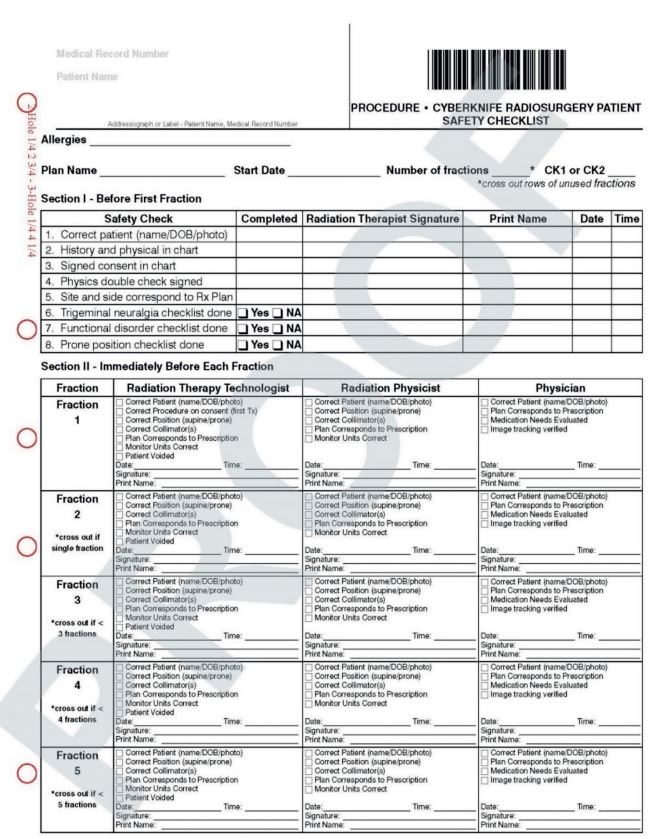
\includegraphics[width=0.9\textwidth]{Imagens/srsChecklistPretratamento.JPG}
		}%
		\caption{Exemplo de um checklist de pré-tratamento para um tratamento SRS/SBRT com multifrações.}
		\label{fig:srsChecklistPretratamento}
	\end{figure}

	O AAPM TG-101 recomenda a documentação de interrupções de tratamento ou desvios no intervalo de tempo de fracionamento pretendido e também recomenda que o físico esteja presente durante todo o primeiro procedimento de tratamento para supervisão e para fornecer supervisão direta para frações subsequentes.

	Atualmente, não existe um guideline uniforme para a supervisão de médicos e físicos durante a administração do tratamento. Os requisitos de supervisão podem ser separados em três níveis:

	\begin{enumerate}[label=\textcolor{CarnationPink}{\arabic*${}^\circ$}]
		\item Requisitos legais definidos por regulamentos federais ou estaduais, requisitos especificados em códigos de faturamento;
		\item Exigências por órgãos de credenciamento (se aplicável);
		\item Recomendações de melhores práticas conforme especificado nas recomendações da sociedade e políticas e procedimentos institucionais.
	\end{enumerate}

	Após a conclusão do tratamento do paciente, uma revisão final formal do prontuário deve ser realizada pelo técnico de radioterapia, físico médico e médico para verificar se o tratamento foi administrado conforme pretendido, se quaisquer desvios do protocolo de tratamento foram documentados e se as instruções/consultas de acompanhamento estão no prontuário.


\bibliography{ref.bib}
\end{document}